\documentclass[12pt]{article}


%Preamble
\usepackage{amsmath}
\usepackage{amssymb}
\usepackage{amsthm}
\usepackage{amsrefs}
\usepackage{amsfonts}
%\usepackage{dsfont}
\usepackage{mathrsfs}
\usepackage{mathtools}
%\usepackage{stmaryrd}
%\usepackage[all]{xy}
\usepackage{enumerate}
\usepackage[shortlabels]{enumitem}
\usepackage{hyperref}
\usepackage[capitalize]{cleveref}
\usepackage{caption, subcaption, tikz}
\usepackage{graphicx}
\graphicspath{{Images/}}
\usepackage{pgfplots}
\usetikzlibrary{arrows}
\usepackage{verbatim} %%includes comment environment
\usepackage{fullpage} %%smaller margins
\usepackage{enumerate}
\usepackage{mathrsfs}

%% Sectioning, Header / Footer, ToC

\usepackage{titlesec}
\usepackage{fancyhdr}
\usepackage{tocloft}

\pgfplotsset{compat=newest,compat/show suggested version=false}

\hypersetup{
    linktoc=all,     %set to all if you want both sections and subsections linked
}

\newcommand{\bbF}{\mathbb{F}}
\newcommand{\bbN}{\mathbb{N}}
\newcommand{\bbQ}{\mathbb{Q}}
\newcommand{\bbR}{\mathbb{R}}
\newcommand{\bbZ}{\mathbb{Z}}
\newcommand{\bbC}{\mathbb{C}}
\newcommand{\abs}[1]{ \left| #1 \right| }
\newcommand{\diff}[2]{\frac{d #1}{d #2} }
\newcommand{\norm}[1]{ \left|\left| #1 \right|\right| }
\newcommand{\eval}[1]{ \left. #1 \right| }

\renewcommand{\phi}{\varphi}

%--------Theorem Environments--------
%theoremstyle{plain} --- default
\newtheorem{thm}{Theorem}[section]
\newtheorem{cor}[thm]{Corollary}
\newtheorem{prop}[thm]{Proposition}
\newtheorem{lem}[thm]{Lemma}
\newtheorem{conj}[thm]{Conjecture}
\newtheorem{quest}[thm]{Question}

\theoremstyle{definition}
\newtheorem{defn}[thm]{Definition}
\newtheorem{defns}[thm]{Definitions}
\newtheorem{con}[thm]{Construction}
\newtheorem{exmp}[thm]{Example}
\newtheorem{exmps}[thm]{Examples}
\newtheorem{notn}[thm]{Notation}
\newtheorem{notns}[thm]{Notations}
\newtheorem{addm}[thm]{Addendum}
\newtheorem{exer}[thm]{Exercise}
\newtheorem{app}[thm]{Application}


\theoremstyle{plain}
\newtheorem{rem}[thm]{Remark}
\newtheorem{rems}[thm]{Remarks}
\newtheorem{warn}[thm]{Warning}
\newtheorem{sch}[thm]{Scholium}

\makeatletter
\let\c@equation\c@thm
\makeatother
\numberwithin{equation}{section}

\bibliographystyle{plain}

%% Sectioning Aesthetics
\titleformat{\section}
{\normalfont\LARGE\bfseries}{\thesection.}{1em}{}
\titleformat{\subsection}
{\normalfont\Large\bfseries}{\thesubsection}{1em}{}
\titleformat{\subsubsection}
{\normalfont\normalsize\bfseries}{\thesubsubsection}{1em}{}
\titleformat{\paragraph}[runin]
{\normalfont\normalsize\bfseries}{\theparagraph}{1em}{}
\titleformat{\subparagraph}[runin]
{\normalfont\normalsize\bfseries}{\thesubparagraph}{1em}{}


%% Header Aesthetics
\pagestyle{fancy}

\setlength{\headheight}{15pt}
\setlength{\headsep}{0.3in}
\renewcommand{\headrulewidth}{0.4pt}
\renewcommand{\footrulewidth}{0.4pt}
\renewcommand{\contentsname}{\hfill\bfseries\Large Table of Contents\hfill}
\renewcommand{\sectionmark}[1]{\markright{ #1}}

\rhead{Marlin Figgins} % controls the left corner of the header
\lhead{\textbf{A Calculus Companion}} % controls the center of the header
\chead{\fancyplain{}{\rightmark}}
 % controls the right corner of the header
\lfoot{Last updated: \today} % controls the left corner of the footer
\cfoot{} % controls the center of the footer
\rfoot{Page~\thepage} % controls the right corner of the footer


\title{\bfseries\huge{A Calculus Companion}\vspace{-1ex}}\author{\href{mailto:figgins.marlin02@gmail.com}{\Large{Marlin Figgins}}\vspace{-2ex}}
\date{August 17, 2018}


\begin{document}

%% Title page with Introduction.
\maketitle
\section*{\hfill Introduction \hfill}
These notes are written as an introduction to calculus. Ideally this is meant to accompany a calculus course like that of MATH 13100-13200-13300 or MATH 15100-15200-15300 at the University of Chicago but can also be used for independent study. I will try my best to balance the theory behind calculus with my use of examples. I admit that my main purpose is to motivate calculus as a tool and develop the theory in accessible language. Most importantly, I hope provide the intuition necessary to understand calculus and its various concepts, so there may not be a ton of examples outside of those necessary to emphasize the thought process behind solving problems with calculus. In the future, I will provide exercises at the end of each section!

\thispagestyle{empty}

%% Table of Contents Page/
\newpage
\tableofcontents
\thispagestyle{empty}
\newpage

%% Set first page after ToC
\setcounter{page}{1}

\section{What is calculus? Why are you learning it?}

The word \emph{calculus} comes from Latin, literally meaning `small pebble', which frankly isn't too far off from the actual concern of calculus. In short, calculus is concerned with two main questions:

\begin{quest}[The Two Main Questions of Calculus]\label{mainquestion}\leavevmode
	\begin{enumerate}
		\item What does a small change in one thing tell you about change in something else?
		\vspace{2mm}
		\item How do these small changes add up to give a sum?
	\end{enumerate}
\end{quest}
We will answer the first of \cref{mainquestion} by learning about something called \emph{differentiation} and the second with another concept called \emph{integration}. As we will see, both questions of \cref{mainquestion} are intimately related, and we'll be able to find a very useful relationship between differentiation and integration.

Before we can even get into answering the two previous questions, we must answer some that you may already have.

\begin{quest}
Why am I learning this?	Why is any of this useful?
\end{quest}

The concepts of differentiation and integration have numerous applications in statistics, physics, chemistry, biology, economics, and generally are useful for understanding how things change in the world around us. In fact, some of the things in the world around you (like your brain, car, and phone) are already using calculus and its principles.

Calculus is used to calculate energy and motion in physics, reaction rates and radioactive decay in chemistry, birth and death rates in biology, and costs and revenues in economics.

Here's an example of a scenario where some of the   central ideas of calculus naturally appear.

\begin{exmp}
Suppose two people $M$ and $J$ are having a race from a point $a$ to another point $b$ and you wanted to know how fast they were going at some point in time $t^*$. We want to look at where they are at different times.

\begin{figure}[h]\label{fig:Race}
\centering
\begin{subfigure}{\textwidth}
  \centering
  \begin{tikzpicture}[scale=.6]
      \draw [very thick] (0,0)-- (16,0);
  		\draw [thick] (0,-.1) node[below]{$a$} -- (0,0.1);
  		\draw [thick] (16,-.1) node[below]{$b$} -- (16,0.1);
  		\draw [thick] (8,-.1) node[below]{$c$} -- (8,0.1);
  		\draw [fill=blue] (0,.5) circle [radius=0.1]
  		node[left] (0, .5) {$J$};
  		\draw [fill=green] (0,1) circle [radius=0.1]
  			node[left] (0, 1) {$M$};
  	\end{tikzpicture}\hspace{12pt}
\end{subfigure}

\begin{subfigure}{\textwidth}
  \centering
\begin{tikzpicture}[scale=.6]
	\draw [very thick] (0,0)-- (16,0);
	\draw [thick] (0,-.1) node[below]{$a$} -- (0,0.1);
	\draw [thick] (16,-.1) node[below]{$b$} -- (16,0.1);
	\draw [thick] (8,-.1) node[below]{$c$} -- (8,0.1);
	\draw [fill=blue] (1,.5) circle [radius=0.1]
	node[left] (1, .5) {$J$};
	\draw [fill=green] (2,1) circle [radius=0.1]
		node[left] (2, 1) {$M$};
\end{tikzpicture}
\end{subfigure}

\begin{subfigure}{\textwidth}
  \centering
\begin{tikzpicture}[scale=.6]
	\draw [very thick] (0,0)-- (16,0);
	\draw [thick] (0,-.1) node[below]{$a$} -- (0,0.1);
	\draw [thick] (16,-.1) node[below]{$b$} -- (16,0.1);
	\draw [thick] (8,-.1) node[below]{$c$} -- (8,0.1);
	\draw [fill=blue] (4,.5) circle [radius=0.1]
	node[left] (4, .5) {$J$};
	\draw [fill=green] (4,1) circle [radius=0.1]
		node[left] (4, 1) {$M$};
\end{tikzpicture}
\end{subfigure}


\begin{subfigure}{\textwidth}
  \centering
\begin{tikzpicture}[scale=.6]
	\draw [very thick] (0,0)-- (16,0);
	\draw [thick] (0,-.1) node[below]{$a$} -- (0,0.1);
	\draw [thick] (16,-.1) node[below]{$b$} -- (16,0.1);
	\draw [thick] (8,-.1) node[below]{$c$} -- (8,0.1);
	\draw [fill=blue] (9,.5) circle [radius=0.1]
	node[left] (9, .5) {$J$};
	\draw [fill=green] (6,1) circle [radius=0.1]
	node[left] (6, 1) {$M$};
\end{tikzpicture}
\end{subfigure}

\begin{subfigure}{\textwidth}
  \centering
  \begin{tikzpicture}[scale=.6]
	\draw [very thick] (0,0)-- (16,0);
	\draw [thick] (0,-.1) node[below]{$a$} -- (0,0.1);
	\draw [thick] (16,-.1) node[below]{$b$} -- (16,0.1);
	\draw [thick] (8,-.1) node[below]{$c$} -- (8,0.1);
	\draw [fill=blue] (16,.5) circle [radius=0.1]
	node[left] (16, .5) {$J$};
	\draw [fill=green] (8,1) circle [radius=0.1]
	node[left] (8, 1) {$M$};
\end{tikzpicture}
\end{subfigure}
\caption{Visualizing the race}
\end{figure}

If we look at \cref{fig:Race}, we see an example of a race like this. In this case, $J$ wins the race in 5 seconds and $M$ loses it, so intuitively, $J$ must have moved faster than $M$. We can attempt to capture this using the average speed formula
\begin{equation}
	\text{Average Speed}=\frac{\text{Distance Traveled}}{\text{Time}}.
\end{equation}
   If we call the speed of $M$ $v_M$ and the speed of $v_J$, then we  have speeds
\begin{equation}
v_M=\frac{c-a}{5}\ \text{and}\ v_J=\frac{b-a}{5}.
\end{equation}
This confirms our guess that $J$ was faster at the end of the day, but something is missing here. At first, $J$ is behind $M$ and moving slower, so $J$ is clearly speeding up. It's not moving at a constant speed. Therefore, we can't just say that it's moving at speed $v_M$ at every time $t^*$. Let's try a different approach. First, we visualize the race by graphing their position at every point in time.
\begin{figure}
  \hspace{-5mm}
\begin{subfigure}{0.35\textwidth}
  \centering
  \begin{tikzpicture}[yscale=0.375, xscale=1.5]
\draw (0,16) -- (0,0) -- (4,0);
	\node [left] at (0,0) [left] {$a$};
		\draw [thick] (-0.05,8) node[left]{$c$} -- (0.05,8);
		\draw [thick] (-0.05,16) node[left]{$b$} -- (0.05,16);

		\draw [thick] (0,-0.1) node[below]{$0$} -- (0,0.1);
		\draw [thick] (1,-0.1) node[below]{$1$} -- (1,0.1);
		\draw [thick] (2,-0.1) node[below]{$2$} -- (2,0.1);
		\draw [thick] (3,-0.1) node[below]{$3$} -- (3,0.1);
		\draw [thick] (4,-0.1) node[below]{$4$} -- (4,0.1);

	\node [right] at (4,0) [right] {$t$};
  \node [above] at (0,16) [above] {$x$};


	\draw[blue, ultra thick, domain=0:4] plot (\x, {\x*\x});

	\draw[green, ultra thick, domain=0:4] plot (\x, {2*\x});

	\node at (2,4) [right] {$x_M(2)=x_J(2)$};
	\node at (4,8) [right] {$x_M(4)$};
	\node at (4,16) [right] {$x_J(4)$};

	\draw[fill] (0,0) circle [radius=0.05];
	\draw[fill] (2,4) circle [radius=0.05];
	\draw[fill] (4,8) circle [radius=0.05];
	\draw[fill] (4,16) circle [radius=0.050];
\end{tikzpicture}
\end{subfigure}
\hspace{35mm}
\begin{subfigure}{0.35\textwidth}
  \centering
  \begin{tikzpicture}[scale=13, yscale=0.6, xscale=2.2]
  	\draw (1.9, 4.41)-- (1.9,3.61)-- (2.1,3.61);

  	\node at (1.9, 3.6) [below] {$1.9$};
  	\node at (2, 3.61) [below] {$2.0$};
  	\node at (2.1, 3.61) [below] {$2.1$};
  	\node at (1.895, 3.61) [left] {$3.61$};
  	\node at (1.895, 3.8) [left] {$3.80$};
  	\node at (1.895, 4) [left] {$4.00$};
  	\node at (1.895, 4.2) [left] {$4.20$};
  	\node at (1.895, 4.41) [left] {$4.41$};
  	\node at (2.105, 3.61) [right] {$t$};


  \draw (1.895, 3.8)-- (1.905, 3.8);
  \draw (1.895, 4)-- (1.905, 4);
  \draw (1.895, 4.2)-- (1.905, 4.2);
  \draw (1.895, 4.41)-- (1.905, 4.41);
  \draw[thick] (2, 3.605)-- (2, 3.615);
  \draw[thick] (2.1, 3.605)-- (2.1, 3.615);


  	\draw[blue, thick, domain=1.9:2.1] plot (\x, {\x*\x});
  	\draw[green, thick, domain=1.9:2.1] plot (\x, {2*\x});
  \end{tikzpicture}
\end{subfigure}



\caption{Graph of time $t$ v. position $x$ at different scales.}
\end{figure}


From this, we see that the position of $M$ and $J$ are functions of time. We'll denote these position functions by $x_M$ and $x_J$. This allows us to rephrase the question. If we want to figure out how fast $M$ and $J$ moving at $t^*$, we need to see how their position functions change around $c$. We want  the rate of change of $x_M$ and $x_J$ around $t^*$. In algebra 1 or 2, you learn to calculate rate of change as the slope of a line $y=mt+b$.
\begin{equation*}
	\text{Rate of Change}=\frac{\text{Change in}\ y  }{\text{Change in}\ t}.
\end{equation*}
We'll write these changes as $\Delta y$ and $\Delta t$. If we zoom in on our functions $x_J$ and $x_M$ far enough, we see that they look straight lines. This allows us to look at small differences in $t$, $x_M$, and $x_J$. Let's say $x_M(2.1)=4.2$, $x_M(1.9)=3.8$, $x_M(2.1)=4.41$, and $x_M(1.9)= 3.61$. If we try to approximate the rate of change this way, then the velocity of $M$ and $J$ at $t^*=2$ are approximately given by: \begin{align}
	v^*_M\approx&\frac{\Delta x_M}{\Delta t}=\frac{4.2-3.8}{2.1-1.9}=\frac{0.4}{0.2}=2\\
	v^*_J\approx&\frac{\Delta x_J}{\Delta t}=\frac{4.41-3.61}{2.1-1.9}=\frac{0.8}{0.2}=4.
\end{align}

We now know that if we zoom in very close and look at small differences, then we're able to approximate how something is changing at a particular moment. This is the same idea behind how a car's speedometer calculates the speed of the car. Calculus comes in when we try to make this method more generally applicable.
\end{exmp}


\section{Limits and Continuity}

%% Flesh out continuity and add more expositon, provide an involved example of where one might to use a limit

In the previous example, we saw that zooming in and only looking at the average speed for small time intervals can help us figure out the speed at a particular moment in time, but we still don't know exactly how close we have to zoom to guarantee the right answer. This leads us to the concept of limits.\\

Conceptually a limit asks, \emph{what happens to our function when you get very close to a certain point?}. Looking at our previous example, we zoomed in on $t^*$ to find the limit of $\frac{\Delta x}{\Delta t}$ as $\Delta t$ got small or \emph{approaches 0}. This is idea behind a limit. Since the position of the runners changed in time, we were able to `zoom in' on a particular time to find how fast they were moving at that instant.

\subsection{Preliminaries \& Limit Definitions}

Before moving for let's look at this more abstractly and develop some notation for dealing with these questions. From the discussion above, we can see that we're interested in functions of some kind of \emph{variable} like time, position, height, energy, population, dollars or whatever quantity you might think of. That is, if we have a number $x$ representing a quantity like this, we want to assign it to another number $f(x)$.  We'll call the rule $f$ which takes $x\mapsto f(x)$ a \emph{function}. Usually, we'll just write $x\in\bbR$ to say that $x$ is a \emph{real number} like the ones we encounter in everyday life. 1,2,3, $\frac{2}{3}$, 1.21, and 3.14 for example. With this in mind, since the function $f$ takes real numbers to real numbers, we can write it as
\[
f\colon \bbR \to \bbR.
\] Alternatively, if $f$ isn't defined for all numbers $\bbR$, but only some subset of numbers $A$, we can write that $f\colon A\to\bbR$. This means that $f$ takes $x$ in $A$ to $f(x)\in\bbR$. These sets $A$ are usually `nice' sets like \emph{open interval} $(a,b)$ i.e. the set of real numbers that are between $a$ and $b$ or
\[
(a,b)=\{x\in\bbR \mid a<x<b \}
\]
or the closed interval which includes the endpoints
\[
[a,b]=\{x\in\bbR \mid a\leq x\leq b \}.
\]

\begin{rem}
  The brackets $\{\cdot \}$ used above are used to denote a \emph{set} and we often use set notion to denote a `container' of objects as a way of simplify our notion. For example, we'll write $\{y\mid C \}$ to denote the collection of objects $y$ that satisfy a condition $C$. We'll say that $x\in \{y\mid C \}$ to mean that $x$ is an element of our set i.e. that $x$ satisfies the condition $C$. %%Maybe turn into appendix of set notion.
\end{rem}
Let's we reframe this limit idea in this fancy new notation.
If we have a function $f\colon A\to \bbR$ and want to find the limit as $x$ approaches $a$ to exist, then we want $f(x)$ to approach a single number as we get close to our point $a$. In order to get at what this means mathematically, we need something called the \emph{absolute value} or \emph{norm}, which is what mathematicians use to measure magnitudes and distances. As you will see, the absolute value follows most of the same rules you would expect of distances in real life.

\begin{defn}[Absolute Value]
The absolute value of a number $a$ is defined by:
\begin{equation}
	\abs{a}=\begin{cases}
		a &\ \text{if}\ a\geq 0\\
		-a &\ \text{if}\ a<0.
\end{cases}
\end{equation}
\end{defn}

 We can think as the absolute value as function that takes in a number and returns the positive part. For example, $\abs{-3}=3$. In this way, it is similar to distance. In real life, if you move 5 feet to the left or to the right, you still moved 5 feet; the only difference is \emph{direction}. Therefore, the absolute value is only concerned with the \emph{magnitude} or \emph{total distance} traveled by saying that moving 5 feet in any direction is the same in terms of distance. Similarly, we say that the distance between two points $x$ and $a$ is given by $\abs{x-a}$. We can use inequalities to illustrate this. What if I ask you to solve the inequality
 \begin{equation*}
 	\abs{x-4}<7.
\end{equation*}
We can solve this by noticing that if $\abs{x-4}<7$, then both $x-4<7$ and $4-x<7$, so $x-4>-7$. Doing some work with inequalities, we see that
\begin{equation}
  -7<x-4<7
  \implies-3<x<11.
\end{equation}
We can visualize this on a number line.\\
\begin{figure}
  \centering
	\begin{tikzpicture}[scale=0.75]
		\draw[<->] (-6,0) -- (13,0);
	%	\draw[thick] (0,0.1)-- (0,-0.1);
		\draw[thick] (-3,0.1)-- (-3,-0.1);
		\draw[thick] (11,0.1)-- (11,-0.1);
		\draw[thick] (4,0.1)-- (4,-0.1);

		\node at (-3, -0.1) [below] {$-3$};
		\node at (4, 0) [below] {$4$};
		\node at (11, -0.1) [below] {$11$};

		\draw[thick, cyan, (-)] (-3,0) -- (11,0);
	\end{tikzpicture}\caption{$\abs{x-4}<7$ on the number line.}
\end{figure}

The absolute value has several interesting properties that are consistent with our interpretation of it as distance.

\begin{prop}[Properties of Absolute Value]\leavevmode
	For any numbers $x$ and $y$
\begin{enumerate}
	\item $\abs{x}=0$ if and only if $x=0$,
	\item $\abs{x}=\abs{-x}$,
	\item $\abs{xy}=\abs{x}\abs{xy}$,
	\item $\abs{x^2}=\abs{x}^2=x^2$,
	\item $\abs{x+y}\leq\abs{x}+\abs{y}$.
\end{enumerate}
\end{prop}

The last property is called the \emph{triangle inequality} and will prove to be very useful in establishing some of the properties of limits.\\

%% Add more about absolute value

%% Do one more example and add two exercises?


With an idea of distance and closeness at hand, we can revisit the question of \emph{what happens to our function when you get very close to a certain point?}. Let's say we have a function $f\colon A\to \bbR$ and a point $a$. If we want to find the \emph{limit of $f$ as $x$ approaches $a$}, we want to find a number $L\in\bbR$ such that \emph{$f(x)$ approaches $L$ when $x$ approaches $a$}. If we can find a number like this, we write
\begin{equation}
	\lim_{x\to a}f(x)=L.
\end{equation}
\begin{defn}\label{EpsDeltaDef}
	Formally, we define this by
	\begin{equation}
		\lim_{x\to a}f(x)=L
	\end{equation}
if for every $\epsilon>0$, there exists $\delta>0$ such that
\begin{equation*}
\abs{x-a}<\delta \implies \abs{f(x)-L}< \epsilon.
\end{equation*}
\end{defn}
\begin{rem}
  In words, we would say `the limit of $f$ as $x$ approaches $a$ is equal to $L$'.
\end{rem}

This is an example of a `$\epsilon$-$\delta$' statement which can be very difficult to unpack when you first see.To help give the notation above meaning, we attempt to visualize this $\epsilon$-$\delta$ definition of a limit in \cref{fig:EpDelta} below.

\begin{figure}\label{fig:EpDelta}
\centering
\hspace{-6mm}
\begin{subfigure}{0.35\textwidth}
  \centering
  \begin{tikzpicture}[scale=.5]
    \draw [<->] (0,10)--(0,0)-- (10,0);
    \draw[thick] (5, 0.1) -- (5, -0.1);
    \draw[thick] ( 0.1,5) -- (-0.1,5);
    \draw[thick, cyan, (-)] (0,4)--(0,6);

\node at (5,0) [below] {$a$};
\node at (0,5) [left] {$L$};
\node at (0,4) [left] {$L-\epsilon$};
\node at (0,6) [left] {$L+\epsilon$};

\draw[dashed] (0,4)-- (10,4);
\draw[dashed]	(0,6)-- (10,6);

\draw[thick, domain=0:7.5] plot (\x, {\x});
\draw[fill=white] (5, 5) circle [radius=0.2];
  \end{tikzpicture}
  \caption{For every $\epsilon>0$,}
\end{subfigure}\hfill%
\begin{subfigure}{0.35\textwidth}
  \centering
\begin{tikzpicture}[scale=.5]
	\draw [<->] (0,10)--(0,0)-- (10,0);
	\draw[thick] (5, 0.1) -- (5, -0.1);
	\draw[thick] ( 0.1,5) -- (-0.1,5);
	\draw[thick, cyan, (-)] (0,4)--(0,6);
  \draw[thick, cyan, (-)] (3,0)--(7,0);

\node at (5,0) [below] {$a$};
\node at (0,5) [left] {$L$};
\node at (3,0) [below] {$a-\delta$};
\node at (7,0) [below] {$a+\delta$};

\draw[dashed] (0,4)-- (10,4);
\draw[dashed]	(0,6)-- (10,6);

\draw[thick, domain=0:7.5] plot (\x, {\x});
\draw[fill=white] (5, 5) circle [radius=0.2];
\end{tikzpicture}
\caption{there exists $\delta>0$ such that}
\end{subfigure}
\vspace{5mm}
\begin{subfigure}{0.35\textwidth}
  \centering
\begin{tikzpicture}[scale=.5]
	\draw [<->] (0,10)--(0,0)-- (10,0);
	\draw[thick] (5, 0.1) -- (5, -0.1);
	\draw[thick] ( 0.1,5) -- (-0.1,5);
	\draw[thick, cyan, (-)] (0,4)--(0,6);
	\draw[thick, cyan, (-)] (3.5,0)--(6.5,0);

	\draw[thick] (4.3, 0.1) -- (4.3, -0.1);
	\node at (4.3, 0) [below] {$x$};
	\draw[dashed] (3.5,0)-- (3.5,10);
	\draw[dashed]	(6.5,0)-- (6.5,10);
	\draw[dotted] (4.3,0)-- (4.3, 10);

	\node at (5,0) [below] {$a$};
	\node at (0,5) [left] {$L$};

	\draw[dashed] (0,4)-- (10,4);
	\draw[dashed]	(0,6)-- (10,6);

	\draw[thick, domain=0:7.5] plot (\x, {\x});
	\draw[fill=white] (5, 5) circle [radius=0.2];
\end{tikzpicture}
\caption{if $\abs{x-a}<\delta$, }
\end{subfigure}\hfill%
\begin{subfigure}{0.35\textwidth}
  \centering
  \begin{tikzpicture}[scale=.5]
  		\draw [<->] (0,10)--(0,0)-- (10,0);
  		\draw[thick] (5, 0.1) -- (5, -0.1);
  		\draw[thick] ( 0.1,5) -- (-0.1,5);
  		\draw[thick, cyan, (-)] (0,4)--(0,6);
  		\draw[thick, cyan, (-)] (3.5,0)--(6.5,0);

  		\draw[thick] (4.3, 0.1) -- (4.3, -0.1);
  		\node at (4.3, 0) [below] {$x$};

  		\draw[dashed] (3.5,0)-- (3.5,10);
  		\draw[dashed]	(6.5,0)-- (6.5,10);
  		\draw[dotted] (4.3,0)-- (4.3, 10);

  		\node at (5,0) [below] {$a$};
  		\node at (0,5) [left] {$L$};

  		\draw[thick] ( 0.1,4.3) -- (-0.1,4.3);
  		\node at (0,4.3) [left] {$f(x)$};

  		\draw[dashed] (0,4)-- (10,4);
  		\draw[dashed]	(0,6)-- (10,6);
  		\draw[dotted] (0,4.3)-- (10, 4.3);

  		\draw[thick, domain=0:7.5] plot (\x, {\x});
  		\draw[fill=white] (5, 5) circle [radius=0.2];
  \end{tikzpicture}
  \caption{then $\abs{f(x)-L}<\epsilon$.}
\end{subfigure}

\caption{Visualizing the $\epsilon$-$\delta$ definition.}
\end{figure}

Intuitively, this is saying that if $\lim\limits_{x\to a}f(x)=L$, then our function $f$ can get close as we want to some value $L$ if we zoom in close enough to $a$ i.e. if $f(x)\approx L$ whenever $x\in(a-\delta,a+\delta)$ for some small number $\delta$.\\

Be fair warned, not all functions have proper limits everywhere! Take
\[
g(x)=\begin{cases}
  1 & \text{if } x\geq 0\\
  0 & \text{if }  x<0,
\end{cases} %% Graph this function below.
\]for example! If we graph this function, we'll see that it clearly has no limit at 0. Before moving on to some of the interesting properties of limit, let's show an example of how to use the $\epsilon-\delta$ definition to prove a limit exists.
\begin{exmp}
  Calculate $\lim\limits_{x\to 2} (3x-1)$ and prove your result. \\

Looking at the graph of $f(x)=3x-1$, you can see that $\lim\limits_{x\to 2} 3x-1=5$, but in order to \emph{prove} this, we must use the $\epsilon$-$\delta$ definition.\\

Suppose we have some small number $\epsilon>0$. If the limit exists, then we know that if we zoom in close enough to $a=2$ on the $x$-axis that our function $f(x)=3x-1$ will be $\epsilon$ close to the limit $L=5$. The point of $\delta$ is to tell us how close we need to be to $a=2$ so that $f(x)=3x-1$ is $\epsilon$-close to $5$. Let's show this mathematically in terms of \cref{EpsDeltaDef}.\\

\begin{figure}
  \centering
\begin{tikzpicture}[scale=.7]
		\draw [<->] (0,10)--(0,0)-- (10,0);
		\draw[thick] (5, 0.1) -- (5, -0.1);
		\draw[thick] ( 0.1,5) -- (-0.1,5);
		\draw[thick, cyan, (-)] (0,4)--(0,6);
		\draw[thick, cyan, (-)] (3.5,0)--(6.5,0);

		\draw[thick] (4.3, 0.1) -- (4.3, -0.1);
		\node at (3.5, 0) [below] {$2-\delta$};
    \node at (6.5, 0) [below] {$2+\delta$};


		\draw[dashed] (3.5,0)-- (3.5,10);
		\draw[dashed]	(6.5,0)-- (6.5,10);
		\draw[dotted] (4.3,0)-- (4.3, 10);

		\node at (5,0) [below] {$2$};
		\node at (0,5) [left] {$5$};

		\node at (0,4) [left] {$f(x)-\epsilon$};

    \node at (0,6) [left] {$f(x)+\epsilon$};

		\draw[dashed] (0,4)-- (10,4);
		\draw[dashed]	(0,6)-- (10,6);
		\draw[dotted] (0,4.3)-- (10, 4.3);

		\draw[thick, domain=0:7.5] plot (\x, {\x});
		\draw[fill=white] (5, 5) circle [radius=0.2];
\end{tikzpicture}
\caption{Visualizing the argument above.}
\end{figure}

We see that if $f(x)$ is $\epsilon$-close to $5$, we can write this mathematically as
\[
\abs{f(x)-5}<\epsilon.
\]
If we substitute in the definition of $f(x)$, we see
\[
\abs{(3x-1)-5}=\abs{3x-6}<\epsilon,
\]
but what we want to find is a number $\delta$, so that if $x$ is $\delta$-close then $f(x)$ is $\epsilon$-close to 5! We can write $x$ is $\delta$-close to $2$ as
\[
\abs{x-2}<\delta.
\]
If you compare the two inequalities above, you see that you can make the lefthand sides equal by multiplying by $3$ which shows
\[
3\abs{x-2}= \abs{3x-6}=\abs{3x-1)-5} <3\cdot\delta.
\]
From this, we see that if $\delta=\frac{\epsilon}{3}$, then
\[
\abs{3x-6}<3\cdot\delta=3\cdot\frac{\epsilon}{3}=\epsilon,
\]
which gives us the inequality we want to see! With this information, we can write the proof as follows.
\begin{proof}
  Let $\epsilon>0$ and $\delta=\frac{\epsilon}{3}$. If
  \[
\abs{x-2} < \delta,
  \]
  then after multiplying by 3, we see
  \[
\abs{3x-6} < \epsilon.
  \]
  Therefore,
  \[
    \abs{3x-6}=\abs{(3x-1)-5} =\abs{f(x)-5 }<\epsilon,
    \]
which proves that the limit is equal to 5.
\end{proof}
\end{exmp}


%% Add left hand and right hand limits


%% A limit exists if and only if the left and righthand limits exist and are equal

%% \begin{thm}
%%  If $\lim\limits_{x\to a^{-}}f(x)=L$ and $\lim\limits_{x\to a^{+}}f(x)=L$, then $\lim\limits_{x\to a}f(x)=L$
%% \end{thm}

%% Piecewise example

%% Difference between limit DNE and function undefined

The idea of limits is conceptually robust and natural, but when it comes to most of applications we're interested in, we'll encounter more complicated functions which make this approach either extremely difficult or just tedious. Because of this,  we'll develop some methods of computing complicated limits using simpler functions which we already know the limit of. For example, if we have two functions $f$ and $g$ which have limits $L$ and $M$, it's reasonable to assume that $f+g$ converges to $L+M$ (why?). Is this also true for $f\cdot g$ or $10\cdot f$? We'll provide an answer to these questions with the following with the following theorems.

\subsection{Limit Theorems}

\begin{thm}[Properties of Limits]\label{LimRules}
If the limits of two functions $f(x)$ and $g(x)$ exist at $a$. That is, if $\lim\limits_{x\to a}f(x)=L$ and $\lim\limits_{x\to a}g(x)=M$ for some numbers $L$ and $M$, then
	\begin{enumerate}
		\item $\lim\limits_{x\to a}\left[f(x)+g(x)\right]=L+M$,
		\item $\lim\limits_{x\to a}\left[cf(x)\right]=cL$ if $c$ is any number,
		\item  $\lim\limits_{x\to a}\left[f(x)\cdot g(x)\right]=L\cdot M$,
		\item if $M\neq 0$, $\lim\limits_{x\to a}\frac{f(x)}{g(x)}=\frac{L}{M}$.
		\end{enumerate}
\end{thm}

As you can see, these rules make calculating limits like
\begin{equation}
\lim\limits_{x\to 3}\frac{x^2-1}{x^8-3x}
\end{equation}
much easier. In this case, it's as simple as plugging in 3 into our equation, but it won't always be this easy. We'll formalize this idea of functions are `nice' and  `not-so-nice' to evaluate with limits in the next sections as we develop the ideas of \textit{continuity} and \textit{differentiblity}.\\

%% Move onto the left and right hand derivatives?

Conceptually, we say that a function is continuous if we `can draw its graph without lifting our pencil`, but mathematically this means that if we move a tiny little on the $x$-axis then we also move a tiny bit up or down on the graph of our function. Let's try and write this idea in terms of limits.

\begin{defn}
We say that a function $f(x)$ is \emph{continuous at $a$} if \begin{equation}
	\lim\limits_{x\to a}f(x)=f(a).
\end{equation}
If $f(x)$ is continuous at every point it is defined, then we just say that $f(x)$ is continuous.
\end{defn}

As you might expect, not all functions are continuous, take $\frac{1}{x}$ for example. This fails to be continuous at $0$.

The limit properties described earlier are useful for determining continuity.
\begin{thm}
	If $f$ and $g$ are continuous at $a$, then
	\begin{enumerate}
		\item $f+g$, $f\cdot g$ are continuous at $a$,
		\item $cf$ is continuous at $a$ for any real number $c$,
		\item $\frac{f}{g}$ is continuous at $a$ whenever $g(a)\neq 0$.
	\end{enumerate}
\end{thm}

We also have another property for the composition of continuous functions.

\begin{thm}
	If $f$ is continuous at $a$ and $g$ is continuous at $f(a)$, then $g\circ f$ is continuous at $a$.
\end{thm}


There are other properties of limits and continuity such as the squeeze and intermediate value theorems! We'll begin with the squeeze theorem.

\begin{thm}[Squeeze Theorem]
  Suppose $f(x)$ is defined near $c$, and there are functions $U(x)$ and $L(x)$ which bound $f(x)$ near $c$ i.e.
  \[
L(x)\leq f(x)\leq U(x)\text{ for every }x\text{ near }c.
  \]
  If $\lim\limits_{x\to c} U(x)= \lim\limits_{x\to c} L(x)$, then
  \[
  \lim\limits_{x\to c} L(x)=\lim\limits_{x\to c} f(x) =\lim\limits_{x\to c} U(x).
  \]
\end{thm}

  This is the statement that if $f(x)$ is sandwiched between two functions $L(x)$ and $U(x)$ that approach each other, then $f(x)$ must approach their common value. We can see an application of this theorem in the following example.

  \begin{figure}[h]
    \centering
    \begin{tikzpicture}
    \begin{axis}[samples=500,domain=-1:1,restrict y to domain =-1:1]
    \addplot[thick,blue ]plot (\x, {0.98*\x*sin(pow(\x,-2) r)});
    \addplot[thick,green]plot (\x, {abs(\x)});
    \addplot[thick,red]plot (\x, {-abs(\x)});
    \end{axis}
    \end{tikzpicture}
    \label{fig:Squeeze}
    \caption{Graphs of $f(x)=x\sin\left(\frac{1}{x^2}\right), L(x)=-\abs{x}|, U(x)=\abs{x}$.}
  \end{figure}


\begin{exmp}
  What is the limit of $f(x)=x\sin\left(\frac{1}{x^2}\right)$ as $x$ approaches 0?\\

  Graphing the function ( \cref{fig:Squeeze}), we see that as we zoom into the origin, $f(x)$ appears to approach zero. We can see this analytically by considering the absolute value of $f(x)$ as follows

  \begin{align}
    \abs{f(x)}&=\abs{x\sin\left(\frac{1}{x^2}\right) }\\
    &= \abs{x}\cdot\abs{\sin\left(\frac{1}{x^2}\right) }.
  \end{align}

The part of interest here is the $\sin\left(\frac{1}{x^2}\right)$. One might remember from pre-calculus that $\sin(\theta)$ is bounded between $1$ and $-1$ for every number $\theta$. Therefore, we see that
\[
\abs{f(x)}\leq \abs{x}\text{ for any }x \text{ near }0.
\]
Breaking down the absolute value around $f(x)$, then gives us

\[
-\abs{x}\leq f(x)\leq \abs{x}\text{ for any }x \text{ near }0.
\]
Therefore, we have functions $U(x)=\abs{x}$ and $:(x)=-\abs{x}$ such that
\[
\lim\limits_{x\to 0} U(x)=\lim\limits_{x\to 0} L(x)= 0
\]
which bound $f(x)$ near 0. Therefore, by Squeeze Theorem, we now know that
\[
\lim\limits_{x\to 0}x\sin\left(\frac{1}{x^2}\right)=0.
\]
\end{exmp}

Another useful theorem involving limits and continuity is the Intermediate Value Theorem!

\begin{thm}[Intermediate Value Theorem]
  Suppose $f$ is continuous on an interval $[a,b]$ and $M$ is a number between $f(a)$ and $f(b)$, then there is some point $c$ between $a$ and $b$ such that $f(c)=M$.
\end{thm}
The intuition behind this relies on the fact that if a function is continuous, then it has no `hops,skips, breaks, or jumps'. Therefore, for a continuous function to go from greater than $M$ to less than $M$, the function must pass through $M$ at some point!\\

We can use the Intermediate Value Theorem to show the existence of roots for a given function.

\begin{exmp}
Show that $f(x)=3x^3+x^2-x-\frac{1}{8}$ has a root.\\

\begin{figure}
  \centering
  \begin{tikzpicture}[scale=0.75]
  \begin{axis}[samples=500,domain=-1:1,restrict y to domain =-1.25:3]
  \addplot[thick,blue ]plot (\x, {3*\x*\x*\x+\x*\x-\x-1/8});
  \addplot[thin,black ] plot (\x, {0});
  \end{axis}
  \end{tikzpicture}
  \caption{Graph of $f(x)=3x^3+x^2-x-\frac{1}{8}$ on $[0,1]$}
\end{figure}

Let's consider $f$ on the interval $[-1,1]$. We can compute that $f(-1)=-1-\frac{1}{8}$ and $f(1)=3-\frac{1}{8}$. We notice that
\[
f(-1)<0<f(1).
\] Since $f(x)$ is continuous, we can apply the Intermediate Value Theorem which tells us that there is some point $c$ between $0$ and $1$ such that $f(c)=0$. This, however, doesn't answer the question of how many roots $f(x)$ has in $[0,1]$. The Intermediate Value Theorem guarantees that there is at least one root of $f$. If we graph $f(x)$, we see that it actually has 3 roots in $[0,1]$.
\end{exmp}

%% Talk about intermediate value theorem use some polynomial as example of having multiple roots but only showing existence of a root!

%% Let's see another way this can be apply
%% Bower's fixed point theorem if f takes interval to itself it has a fixed points

%% A population grows by ,,,, we want to know if there's a stable population

%% Discrete logistic map, rx(1-x)m we can see that the max of this is r/4

%% Later, we'll be able to show that the maximum is

%% Later, we can see whether or not the population will actually approach the fixed point

%% How does the equilibrium change with the fertility r.


We now move onto the actual definition of differentiability, so that we can answer our question about how to find the rate of change of a function at a given point.

\section{Differentiation}

%% Returning to the problem in first section, we want to answer the question of how fasr x is moving at time 2 .

%% As we saw in figure, we can estimate this by taking closer and closer time and distance measurements,,,

%% We can formalize with a limit


\begin{defn}[Definition of the Derivative]\label{DifDef}
	We say that a function $f$ is \emph{differentiable at $a$} if
	\begin{equation}
		f'(a)\coloneqq\lim\limits_{h\to 0}\frac{f(a+h)-f(a)}{h} \text{ exists}.
	\end{equation}
	We call $f'(a)$ the derivative of $f(x)$ at $a$. If $f$ is differentiable at every point it is defined, we say that $f$ is differentiable and call $f'$ the derivative of $f$.
\end{defn}
\begin{rem}
Alternatively, we may write the derivative of $f$ as $\diff{f}{x}(a)$ or $\diff{}{x}\Big(f(x)\Big)$. Here, $\diff{}{x}$ tells us to take the derivative of $f$.
\end{rem}
Let's unpack this definition. Recall that we can write the formula for a line between two points $(x_1, y_1)$ and $(x_2, y_2)$ as
\[
y_2 - y_1 = m(x_2-x_1)
\]
where $m$ is the slope. In this case, we can calculate the slope of this line as
\[
m = \frac{\Delta y}{\Delta x} = \frac{y_2 - y_1}{x_2 - x_1}
\]
which is the change in $y$ divided by the change in $x$. Substituting this into the point-slope formula, we see that
\[
y_2-y_1 = \underbrace{ \left( \frac{\Delta y}{\Delta x} \right) }_{m}(x_2-x_1).
\]

Now looking at \cref{DifDef}, we see that the quotient
\[
\frac{f(a+h)-f(a)}{h}
\] describes the slope of a line between the points $(a, f(a))$ and $(a+h, f(a+h))$, and we want to see what happens to this quotient as $h$ approaches 0.

\begin{center}
	\begin{tikzpicture}[scale=0.7]
		\draw [<->] (10,0)-- (0,0) -- (0,10);
		\draw[thick, domain=0:10] plot (\x, {.1*\x*\x});
		\draw [thick] (3,-0.1)--(3,0.1);
		\node at (3,-0.15) [below] {$a$};
		\draw [thick] (8,-0.1)--(8,0.1);
		\node at (8.1,0) [below] {$a+h_1$};
		\draw [thick] (6,-0.1)--(6,0.1);
		\node at (6.1,0) [below] {$a+h_2$};
		\draw [thick] (4,-0.1)--(4,0.1);
		\node at (4.1,0) [below] {$a+h_3$};

		\draw [thick] (-0.1, 0.9)--(0.1, 0.9);
		\node at (0,0.9) [left] {$f(a)$};
		\draw [thick] (-0.1, 6.4)--(0.1, 6.4);
		\node at (0,6.4) [left] {$f(a+h_1)$};
		\draw [thick] (-0.1, 3.6)--(0.1, 3.6);
		\node at (0,3.6) [left] {$f(a+h_2)$};
		\draw [thick] (-0.1, 1.6)--(0.1, 1.6);
		\node at (0,1.6) [left] {$f(a+h_3)$};

		\draw [fill=black] (3, 0.9) circle [radius=0.1];
		\draw [fill=black] (8, 6.4) circle [radius=0.1];
		\draw [fill=black] (6, 3.6) circle [radius=0.1];
		\draw [fill=black] (4, 1.6) circle [radius=0.1];
		\draw[dashed, red, thick, domain=2:10] plot (\x, {1.1*\x-2.4});

		\draw[dashed, orange, thick, domain=2:10] plot (\x, {0.9*\x-1.8});

		\draw[dashed, green, thick, domain=2:10] plot (\x, {0.7*\x-1.2});


	\end{tikzpicture}
\end{center}

The picture above shows that as $h$ decreases, $\frac{f(a+h)-f(a)}{h}$ begins to resemble the slope of the line tangent to $f(x)$ at $a$. This shows us that the derivative gives us information about the \emph{rate of change} of a function.\\

Motivated by the above picture, we see that if we let $x=a+h$, then our definition of the derivative is equivalent to the following one.

\begin{defn}[Alternative Definition of the Derivative]
	A function $f(x)$ is differentiable at $a$ if
	\begin{equation}\label{AltDifDefEq}
		\lim\limits_{x\to a}\frac{f(x)-f(a)}{x-a}\ \text{exists.}
	\end{equation}
	As before, we denote the value of this limit by $f'(a)$ or $ \diff{f}{x}(a)$.
\end{defn}
\begin{rem}
  Borrowing the notation above, we can write $\Delta f = f(x) - f(a)$ and $\Delta x = x-a$, so that  \eqref{AltDifDefEq} above becomes
  \[
	\lim\limits_{x\to a}\frac{\Delta f}{\Delta x} = \diff{f}{x}(a).
  \]
\end{rem}

%% Example here

Instead of taking the derivative at every single point $a$ that we're interested in, we can try to write the derivative of a function $f(x)$ as another function instead of fixing some point $a$! We can try an example of this.

\begin{exmp}
  From algebra and geometry, we know that a circle with radius $r$ has area $\pi r^2$. What would we do if we wanted to know how quickly the area of the circle would change if we changed our radius. In this case, we write the area function as $A(r) =  \pi r^2$. This time we use the definition of the derivative (\cref{DifDef}) using a variable $r$ for our radius instead of a single point $a$. Therefore, we can attempt to write the derivative $A'(r)$ as
  \[
  A'(r) = \lim\limits_{h\to 0}\frac{A(x+h)-A(x)}{h}.
  \]
  Using our familiar algebra rules, we can show that $A(r+h) = \pi(r+h)^2 = \pi(r^2 + 2rh + h^2) = \pi r^2 + 2\pi rh + \pi h^2$. Therefore, we can rewrite this limit as
  \begin{align}
  A'(x) & = \lim\limits_{h\to 0}\frac{\pi r^2 + 2\pi rh + \pi h^2 - \pi r^2}{h} =  \lim\limits_{h\to 0}\frac{2\pi rh + \pi h^2}{h}\\
  & = \lim\limits_{h\to 0}\frac{h(2\pi r + \pi h)}{h} = \lim\limits_{h\to 0} 2\pi r + \pi h = 2\pi r.
  \end{align} This shows us that the area of a circle of radius $r$ changes at a rate $2\pi r$. We can see this idea geometrically in ()  One thing that should stand out is that this is the same formula as the circumference $C(r)$ of the circle! Therefore, we showed that
  \[
  \diff{A}{r} = C(r).
  \]  In words, this means that the derivative of the area of a circle with radius $r$ is its circumference! We probably wouldn't have noticed this pattern if we tried to find this derivative for specific points one by one.
\end{exmp}

%% Add figure for this circle with $h$


This technique is useful in a lot more cases, so we'll try to generalize this idea a bit. If we have a function $f(x)$ and can find another function that gives us the derivative of $f$ at any point $x$, we simply call it \emph{the derivative of $f$} (without mentioning a specific point). Keeping our notation consistent, we'll write this function as $f'(x)$ or $\diff{f}{x}$! This can be a little confusing at first, but the point is that the derivative of $f$ at a point $a$ is a number $f'(a)$, and the derivative of $f$ is another function $f'$.

When we write it in this way, we can find that the derivative as we defined it has some very nice properties which will make the actual process computing derivatives much easier. You'll notice that several of the properties shown below resemble properties of limits which makes sense since we defined the derivative in terms of limits. These properties also harken back to the limit properties of continuous functions and later, we'll see that all differentiable functions are also continuous.

\subsection{Differentiation Rules}

%% Flesh out this section. Consider moving things around!! Maybe find more indepth examples and exapnd on expositon

As one might expect, using the definition of the derivative on each and every problem we encounter is tedious, boring, and generally uneventful. In order to get around this, we'll develop some tricks for computing derivatives easily using the derivatives of more `elementary' functions.

\begin{prop}[Scalar multiplication and Sum Rules]\label{SMultSumDiff}
	If $f$ and $g$ are differentiable at $a$ and  $c$ is any real number, then $f+g$ and $c\cdot f$ are differentiable at $a$. Moreover,
	\begin{align}
		 (f+g)'(a)&=f'(a)+g'(a)\ \text{and}\\
		  (c\cdot f)'(a)&=c\cdot f'(a).
	\end{align}
\end{prop}
\begin{proof}
We start with the definition of the derivative and through a short computation see that
\begin{align*}
	\lim\limits_{x\to a}\frac{(f+g)(x)-(f+g)(a)}{x-a}&=	\lim\limits_{x\to a}\frac{f(x) +g(x)-f(a)-g(a)}{x-a}\\
	&=\lim\limits_{x\to a}\frac{f(x)-f(a)+g(x)-g(a)}{x-a}\\
	&=\lim\limits_{x\to a}\frac{f(x)-f(a)}{x-a}+\lim\limits_{x\to a}\frac{g(x)-g(a)}{x-a}\\
	&=f'(a)+g'(a).
\end{align*}
Therefore the derivative $(f+g)'(a)$ exists and equals $f'(a)+g'(a)$. A similar computation shows that $(cf)'(a)=c\cdot f'(a)$.
\end{proof}

\begin{thm}[Product Rule]
	If $f$ and $g$ are differentiable at $a$, then $f\cdot g$ is differentiable at $a$ and \begin{equation}
		(f\cdot g)'=f'(a)\cdot g(a)+f(a)\cdot g'(a).
	\end{equation}
\end{thm}

\begin{thm}[Reciprocal Rule]
If $f(x)$ is differentiable at $a$ and $f(a)\neq 0$, then $g(x)=\frac{1}{f(x)}$ is differentiable at $a$ and
\begin{equation}
g'(a)=-\frac{f'(a)}{f(a)^2}.
\end{equation}
\end{thm}

\begin{cor}[Quotient Rule]
	If $f$ and $g$ are differentiable at $a$ and $g(a)\neq 0$, then $Q(x)=\frac{f(x)}{g(x)}$ is differentiable $a$ and
	\begin{equation}
		Q'(a)=\frac{f'(a)g(a)-f(a)g'(a)}{g(a)^2}.
	\end{equation}
\end{cor}

%% Add the chain rule!!

Now that we have all these rules of differentiation, let's see how we can find the derivatives of a common class of functions.

\begin{quest}
	What is the derivative of a polynomial function
	\begin{equation}
		f(x)=a_nx^n+a_{n-1}x^{n-1}+\dotsb+ a_1x+a_0,
	\end{equation}
	where $n=$ is a positive integer and each $a_i$ is any number?
\end{quest}

Let's start with the simple case where our function is constant.

\begin{prop}
The derivative of a constant function $f(x) =c$ is 0.
\end{prop}

\begin{proof}
If $f$ is constant, then $f(x + h) = f(x) = c$. Therefore,
\[
f'(x) = \lim\limits_{h\to 0} \frac{f(x+h)-f(x)}{h} = 0.
\]
\end{proof}

Moving onto the non-constant polynomials, the scalar multiplication and sum rules from above (\label{SMultSumDiff}) tell us that we only need to be able to find the derivative of each $x^k$ to find the derivative of $f(x)$.

\begin{prop}[Power Rule]\label{PowRule}
	If $f(x)=x^n$ for any non-zero number $n$, then the derivative of $f$ is  $f'(x)=nx^{n-1}$.
\end{prop}
\begin{proof}
	We start with the definition of the derivative and substitute in our function $f$ i.e.
	\begin{equation}
		\lim\limits_{h\to 0}\frac{f(x+h)-f(x)}{h}
=	\lim\limits_{h\to 0}\frac{(x+h)^n-x^n}{h}.
	\end{equation}
	Using the fact that \begin{equation}
		(a+b)^n=\sum^n_{k=0} \binom{n}{k}a^{n-k}b^k=a^n+na^{n-1}b+ \frac{n(n-1)}{2!}a^{n-2}b^2+\dotsb+b^n,
	\end{equation}
	where $\binom{n}{k}=\frac{n!}{k!(n-k)!}$,
	we calculate the limit as follows:
	\begin{align}
		\lim\limits_{h\to 0}\frac{(x+h)^n-x^n}{h}&=\lim\limits_{h\to 0}\frac{(x^n+nx^{n-1}h+ \frac{n(n-1)}{2!}x^{n-2}h^2+\dotsb+h^n)-x^n}{h}\\
	&=\lim\limits_{h\to 0}\frac{nx^{n-1}h+ \frac{n(n-1)}{2!}x^{n-2}h^2+\dotsb+h^n}{h}\\
	& =\lim\limits_{h\to 0} \left[ nx^{n-1}+ \frac{n(n-1)}{2!}x^{n-2}h+\dotsb+h^{n-1}\right] .
	\end{align}
Using the additive and multiplicative properties of limits, we see that
\begin{equation}
	f'(x)=\lim\limits_{h\to 0} \left[nx^{n-1}+ \frac{n(n-1)}{2!}x^{n-2}h+\dotsb+h^{n-1}\right]=nx^{n-1},
\end{equation}
which proves the theorem.
\end{proof}

%% Add proving that the derivative of a constant is zero to the exercises

\begin{exmp}
	Using the power rule, find the derivative of $f(x)=x^2+3x$.
\end{exmp}

%% Finish this example


There are other useful derivative formulas that one should know when doing and learning calculus.

\begin{prop}\label{SinCosExpDif}
  The functions $\sin(x), \cos(x)$ and $e^x$ are differentiable.
  \begin{enumerate}
\item The derivative of $\sin(x)$ is $\cos(x)$,
\item the derivative of $\cos(x)$ is $-\sin(x)$,
\item the derivative of $e^x$ is $e^x$, and
\item the derivative of $\ln(x)$ is $\frac{1}{x}$.
\end{enumerate}
\end{prop}
The proofs for the first two parts rely on the following additive identities of trigonometry:
\begin{align}
   \sin(a+b)&=\sin(a)\cos(b)+\cos(a)\sin(b),\\
   \cos(a+b)&=\cos(a)\cos(b)-\sin(a)\sin(b),
\end{align}
and using the following limit identities,
\begin{equation}
  \lim\limits_{x\to 0}\frac{\cos(x)-1}{x}=0 \text{ and } \lim\limits_{x\to 0}\frac{\sin(x)}{x} =1.
\end{equation}
We'll leave the proof of the first two as an exercise, and we'll prove the third and fourth later when we do implicit differentiation.

Now that we understand how to differentiate function like $x^2$ or $\sin(t)$ as well as their sums, products, and quotients, we can begin to tackle a number of problems. But we've yet to answer how we can differentiate \emph{compositions} of functions like $\sin(t^2)$ or $\cos^3(t) + e^{2t}$. That is, we want to understand how we can differentiate functions within other functions. The first step of this is identifying what is a composition of functions. Say we're given the function $\sin(t^2)$ as above. We can clearly see that this is made up of $t^2$ and the familiar $\sin(x)$. To clarify this notation, we write $f(x) = \sin(x)$ and $g(t) = t^2$.  This way, we can see that choosing $x = g(t)$ allows us to write
\[
f(x) = f(g(t)) = f(t^2) = \sin (t^2).
\]
This still doesn't answer the question of differentiation. Let's set up this question more abstractly. Say we have any function $f(x)$ and another function $g(t)$, then our goal is to find the derivative of its composition,
\[
(f\circ g)'(t) = \frac{df}{dt}.
\]
Going back to most basic idea behind the derivative, we know that $f'(x) = \diff{f}{x}$ tells us the rate of change of $f$ as we move near $x$. Therefore, the derivative $f'(g(t))$ should tell us the rate of change near $g(t)$, but since $g$ itself is a function, we must account for the change in $g(t)$ near $t$ i.e. $\diff{g}{t}$. Since $g$ is acting as our input $x$, we can write its derivative as $\diff{x}{t}$.

DONT DO THIS YOURseLF
\[
\diff{f}{t} = \diff{f}{x} \diff{x}{t}.
\]

Handwavely, but the equation is ...

Write as proposition.

\begin{prop}[The Chain Rule]
If $f$ is differentiable at $g(t)$ and $g$ is differentible at $t$, then the derivative of $f\circ g$ is
\[
(f\circ g)'(t) = g'(t)\cdot f'(g(t)).
\]
\end{prop}
\begin{rem}
I often remember this as `the derivative of the inside function times the outside function'.
\end{rem}
%%% ive sin and cos as exercise with the trig rule and limit rule as hints

%% Differentiation Exercises

\begin{exmps}

Compute the derivative $f'(x)$ for the following functions:
\begin{enumerate}[label=\textbf{Example A.\arabic*.}]
  \addtolength{\itemindent}{2.5cm} % move right
  \item \label{DifEA1} $f(x) = x^5+2x+1$,
  \item \label{DifEA2} $f(x) = \sin^3(x)=\big(\sin(x)\big)^3$,
  \item \label{DifEA3} $f(x) = x^3\sin(x)$,
  \item \label{DifEA4} $f(x) =\frac{5x}{x^2+1}$,
  \item \label{DifEA5} $f(x) = e^{6x}$
  \item \label{DifEA6} $f(x) = x^2e^{2x}$
  \item \label{DifEA7} $f(x) = \frac{1}{x^2}$
  \item \label{DifEA8} $f(x) = e^{-6x}\ln(x)$
\end{enumerate}

\textbf{Example A.1.}

Since we're differentiating a sum, we can take the derivative of each of its parts! Using the power rule (\href{PowRule}), we see that the derivative of $x^5$ is $5x^4$, the derivative of $2x$ is $2$ and the derivative of $1$ is 0. This means that the derivative of $x^5 + 2x + 1$ is given by $5x^4 + 2$.

\textbf{Example A.2.}

This problem is an application of the chain rule (add citation) and the power rule! Using the $\sin(x)$ as the `inside' function ($g(x)$) and $x^3$ as the `outside' function $(f(x))$. Starting with the `outside' function $f$ we use the power rule to show
\[
f(x) = x^3 \xrightarrow{\diff{}{x}} f'(x) = 3x^2.
\] by the power rule. Similarly, the derivative of $g(x) = \sin(x)$ is $g'(x) = \cos(x)$ by \cref{SinCosExpDif}. Following the chain rule formula, we can compute $f'(g(x)) = 3 \sin^2(x)$. Therefore, we write the derivative as $3\cos(x)\sin^2(x)$.

%% Make align for the derivative $\diff{}{x}$ over arrow?
\textbf{Example A.3.}

\textbf{Example A.4.}

\textbf{Example A.5.}

\textbf{Example A.6.}

\textbf{Example A.7.}

\textbf{Example A.8.}

\end{exmps}

The derivative is also useful for answering questions about the average rate of change as well as the maxima and minima.


\subsection{Differentiation Theorems}

\begin{thm}[Rolle's Theorem]
Suppose $f$ is continuous on a closed interval $[a,b]$ and differentiable on the open interval $(a,b)$ and $f(a)=f(b)$, then there is some point $c\in [a,b]$ such that $f'(c)=0$.
\end{thm}

With Rolle's theorem, we can define the following theorem which allows us to relate the secant lines discussed earlier with the derivative.
\begin{thm}[Mean Value Theorem]\label{MVTD}
Suppose $f$ is continuous on a closed interval $[a,b]$ and differentiable on the open interval $(a,b)$, then there is some point $c$ in $[a,b]$ such that
\begin{equation}
	f'(c)=\frac{f(b)-f(a)}{b-a}.
\end{equation}
\end{thm}
\begin{proof}
Let $g(x)=f(x)-\frac{f(b)-f(a)}{b-a}(x-a)$. The function $g$ is differentiable with $g(a)=f(a)$ and $g(b)=f(b)$. Using differentiation rules described earlier,
\begin{equation}
	g'(x)=f'(x)-\frac{f(b)-f(a)}{b-a}.
\end{equation}
Therefore, we can apply Rolle's theorem and see that there is some $c$ such that $g'(c)=0$, so
\begin{equation}
	f'(c)=\frac{f(b)-f(a)}{b-a}.
\end{equation}
\end{proof}

Essentially, this theorem states that the secant line of $f$ at the points $a$ and $b$ has the same slope as the derivative $f$ at some point $c$ or \emph{the average rate of change on $[a,b]$ is realized as the instantaneous rate of change at a point $c$ in $[a,b]$}.

%%%%% Figure showing what this looks like %%%

\section{Applications of Differentiation}

\subsection{Extrema: Maxima and Minima}

This leads us to a very important application of calculus showing the existence of and finding extrema. That is, finding the points at which functions attain their extrema i.e. their maxima or minima.

\begin{defn}
  We say that $f$ has a \emph{local maximum} at $c$ if
  \[
f(c)\geq f(x)\ \text{for all }x\text{ sufficiently close to } c.
  \]
Likewise, we define the \emph{global maximum of $f$} to be the point $c$ such that
\[
f(c)\geq f(x)\ \text{for all }x\text{ where $f$ is defined.}
\]
We can define local and global minima similarly by flipping the inequality.
\end{defn}

One thing to notice is that not all functions have local extrema. For example, take the function
\[
f(x)=x \text{ where } 0<x<1
\] or
\[
f(x)= \begin{cases}
0 \text{ when $x$ is in } \bbQ,  \\
1 \text{ otherwise},
\end{cases}
\] which has no local maxima or minima though every point is an absolute maximum or minimum. Luckily, the Extreme Value Theorem gives us criteria to tell when a function has absolute extrema.

\begin{thm}[Extreme Value Theorem]
  If $f$ is continuous on a closed interval $[a,b]$, then $f$ has both a global maximum and minimum on that interval.
\end{thm}

This gives us a neat answer in the case $f$ is continuous on a closed interval $[a,b]$, but what happens if we further assume that $f$ is differentiable on the open interval $(a,b)$.


Let's consider the function $f(x)=1-x^2$ on the interval $[-1,1]$. Clearly, $f$ is continuous on $[-1,1]$ and differentiable on $(-1,1)$. By the Extreme Value Theorem, you can see that we're guaranteed a maximum and minimum on $[-1,1]$. Graphing the function, we see that the minimum occurs at $x=1,-1$ where $f(x)=0$ and that the maximum occurs at $x=0$ where $f(x)=1$. Let's see what this entails for the derivative of $f$. \\


The derivative of $f(x)$ is $f'(x)=-2x$. From this, we can notice that if $x<0$, then $f'(x)>0$. That is $f(x)$ has a positive slope to its tangent and is \emph{increasing}. Similarly, when $x>0$, $f'(x)<0$ and $f$ is \emph{decreasing}.  Furthermore, $f'(0)=0$ which makes sense since for $f$ to achieve a maximum at 0, it must increase to a point and then decrease from there on for $x$ near 0. This means that not only does $f$ have a global maximum at 0; it also has a local maximum.

%% Graph function above show the tangent line for a decreasing and increasing point and a third at minimum.


Above we used the sign of the derivative $f'$ to determine whether $f$ was increasing or decreasing. In general, this holds for every differentiable function $f$.

\begin{prop}
Given a differentiable function $f$,
\begin{enumerate}
  \item If $f'(x)>0$, then $f$ is increasing at $x$.
  \item If $f'(x)>0$, then $f$ is decreasing at $x$.
\end{enumerate}
\end{prop}

This leaves us to understand the case where $f'(x)=0$. We can begin to describe this case using what is known as the \emph{first derivative test}.

\begin{thm}[First Derivative Test]

\end{thm}

%% Make sure to use the language of stationary and critical points


%% Give example of a function with maximum. Then state that $f'(c)$ must be 0.


%% Use as justification for stating how derivative must change from positive to negative! i.e. first derivative test.

%% State second derivative test.

\subsection{Optimization}

%% General Idea, Examples, hint at Calculus of Variations

%% Use the ellipse example for calculus of variations blog post!

\subsection{Linear Approximations}

By construction, the derivative describes the instantaneous rate of change of a function at a particular point. As we saw, this is the slope of the tangent line at that point. Because of this, the derivative can be used to provide an estimate of what the function is doing near a given points. That is, if we fix a function $f$ and a point $a$ where $f$ is differentible, we can use the derivative $f'(a)$ and its corresponding tangent line to $f$ to approximate the function $f$ at points $x$ near $a$. This process is called \emph{linear approximation}.

%% Lay out the statement and do examples where computing might be hard, compare error.

%% Talk about Euler's method (or Newton's method idk which one it is)... direct towards the will be appendix
\subsection{Implicit Differentiation}

In the cases given previously, we have always been able to isolate our expressions as functions of single variable i.e
\[
f(x)=x^2+5x-3\text{ or }y=\frac{\sin (x+1)}{x^2}.
\]
This may not always be possible or the simplest way to do things! Suppose we're given the equation for a circle centered at the origin with radius 1

\[
x^2+y^2=1.
\]

Yes, it is possible to isolate $y$ and find $y=\pm \sqrt{1-x^2}$, but this leaves two different cases to watch out for when finding the derivative on the circle.\\

Instead, if we remember that $y$ is a function as $x$, we can differentiate this equation without isolating $y$ using the \emph{chain rule} as follows:
\begin{equation}
  \diff{}{x}\big[x^2+y^2=1\big]\implies 2x+2y\diff{y}{x}=0.
\end{equation}
Rearranging this, we see that
\[
\diff{y}{x}=-\frac{x}{y} \text{ where $x,y$ satisfy the equation we started with.}
\]

This technique is called \emph{implicit differentiation} and comes in handy when dealing with complex expressions in terms of both $y$ and $x$. Let's do another example.

\begin{exmp}
  Let's consider the curve given by
\begin{equation}\label{ImplicitFunc1}
  y^3-y = x^3-x\cos(30x).
\end{equation}

Suppose we wanted to find the slope of a point tangent to this curve. Instead of hopelessly trying to simplify this equation to solve for $y$ and differentiate, we can differentiate implicitly. Differentiating \eqref{ImplicitFunc1} with respect to $x$, we get \[
3y^2\diff{y}{x}-\diff{y}{x}=3x^2-\cos(30x)-30x\sin(30x).
\]
Pulling out the $\diff{y}{x}$, we see
\[
\diff{y}{x}=\frac{3x^2-\cos(30x)+30x\sin(30x)}{3y^2-1}.
\]
Notice that this derivative is undefined along the lines $y=\pm\frac{1}{\sqrt{3}}$, which correspond the points where the line tangent to the graph is vertical. Similarly, we can find the points where the slope is horizontal by finding the zeroes of $3x^2-\cos(30x)+30x\sin(30x)$.


\begin{figure}
  \centering
  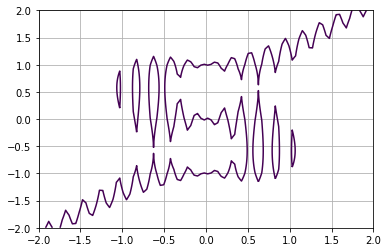
\includegraphics[width=0.4\linewidth]{ImplicitFunc1.png}
  \caption{Graph of (\ref{ImplicitFunc1})}
\end{figure}
\end{exmp}

We can can use implicit differentiation to prove \cref{SinCosExpDif}.3. using \cref{SinCosExpDif}.4.  i.e. that derivative of $f(x)=e^x$ is $e^x$.
\begin{proof}
Suppose we have $y=e^x$. This is equivalent to saying that $\ln y = x$.
Taking the derivative of both sides with respect to $x$, we see that
\[
\frac{1}{y}\diff{y}{x}=1,
\]
using that $\diff{}{y}\left( \ln y \right) = \frac{1}{y}$. Therefoere,
$\diff{y}{x}=y=e^x$.
\end{proof}

\begin{exer}
  Prove that $\diff{}{x}\left( \ln x \right) = \frac{1}{x}$ using that the derivative of $e^x$ is itself.
\end{exer}

\subsection{Related Rates}

\section{Integration}

%% Provide a problem where definite integration is useful,
We'll now begin to develop the concept of \emph{integration}. Where differentiation was concerned with the rate of change at a particular point, integration is concerned with the way these changes accumulate over a range of points. In order to understand this mathematically, we'll need to develop some convenient notion for dealing with sums with a large number of terms. To do this, we'll rely on Riemann sums, but first we'll introduce the ``capital sigma'' notation for sums for those who are unfamiliar.

%%% Starting with defining sum notation

Say we have numbers $a_1, a_2, a_3, a_4$, we can write their sum as $a_1+a_2+a_3+a_4$ or as $\sum_{i=1}^4a_i$ where $i$ is called the `dummy variable'. This is used to make the notation simpler and it'll reoccur often when have many terms to add together. More generally, we can write the sum of numbers $a_1, a_2,\dotsc, a_n$ as
\begin{equation}
\sum_{i=1}^{n}a_i \coloneqq a_1+a_2+\dotsb+a_n.
\end{equation}
One thing to notice is that the sum is \emph{linear}. This property is key to what follows.

\begin{lem}[Linearity of the sum]\label{LinSum}
  For any numbers $a_1, \dotsc a_n$ and $b_1, \dotsc, b_n$ and constant $c$, we have:
  \begin{enumerate}
    \item $\sum_{i=1}^{n}a_i=\sum_{i=1}^{k}a_i+\sum_{i=k+1}^{n}$ for any $k$ between $1$ and $n$,
    \item $\sum_{i=1}^{n}(a_i+b_i)=\sum_{i=1}^{n}a_i+\sum_{i=1}^{n}b_i$,
    \item $\sum_{i=1}^{n}(ca_i)=c\sum_{i=1}^{n}a_i.$
  \end{enumerate}
\end{lem}

%%%% Define linearity of \sum

This linearity also allows us to establish to the following important identities.

\begin{lem}[Formulas for Integer Sums]\label{IntegerSums}
  The following identities hold.
\begin{enumerate}
  \item $\sum_{i=1}^{n}i=\frac{n(n+1)}{2},$
  \item $\sum_{i=1}^{n}i^2=\frac{n(n+1)(2n+1)}{6},$
  \item $\sum_{i=1}^{n}i^3=\left(\frac{n(n+1)}{2} \right)^2.$
\end{enumerate}
\end{lem}
\begin{proof}
  These can be proved by induction using the linearity of the sum as established in \cref{LinSum}.
\end{proof}

\subsection{Riemann Sums}

These identities will be helpful in establishing the integrals in several of the sums that will appear. When we ``integration is concerned with the way changes accumulate'', we often want to this as the integral as the area under the curve of a function over an interval. Therefore, we start by trying to approximate this area under the curve using rectangles as in \cref{fig:RiemannSumIncresN}. In order to this, we have to divide our interval into pieces that will from the bases of these rectangles. This is the idea of the partition.
\begin{defn}[Partition]
If we have an interval $[a,b]$, we define a \emph{partition $P$ of $[a,b]$} to be the set of points $P=\{x_0,x_1,\dotsc, x_n\}$. Additionally, we define the \emph{mesh} of the partition $\abs{\abs{P}}$ to be the maximum length of the intervals $[x_i,x_{i+1}]$ in $P$.
\end{defn}

With partitions under our belt, we can define the Riemann sum: our approximation of the area underneath the curve given a particular partition.

\begin{defn}[Definition of the Riemann Sum]
  Given a function $f$ on the interval $[a,b]$ and a partition $P=\{x_0,x_1,\dotsc, x_n\}$ of [a,b], we define the \emph{upper Riemann sum of $f$ with respect to $P$} as
\begin{equation}
  U(f;P)\coloneqq\sum_{i=1}^{n}f(x_i)(x_i-x_{i-1}).
\end{equation}
Similarly, we can define the \emph{lower Riemann sum} as
\begin{equation}
  L(f;P)\coloneqq\sum_{i=1}^{n}f(x_{i-1})(x_i-x_{i-1}).
\end{equation}
Between this two, we can also define the \emph{ midpoint Riemann sum} by taking the midpoints of each interval, so that
\begin{equation}
  M(f;P)\coloneqq\sum_{i=1}^{n}f\left(\frac{x_{i}+x_{i-1}}{2}\right)(x_i-x_{i-1}).
\end{equation}
\end{defn}

\begin{figure}
\centering
\begin{subfigure}{.33\textwidth}
  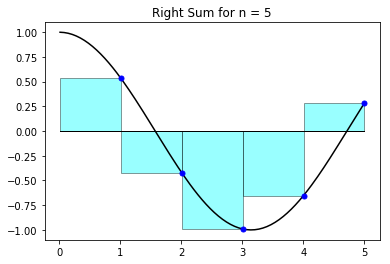
\includegraphics[width=0.9\linewidth]{RiemannSumN5.png}
  \caption{n=5}
\end{subfigure}%
\begin{subfigure}{.33\textwidth}
  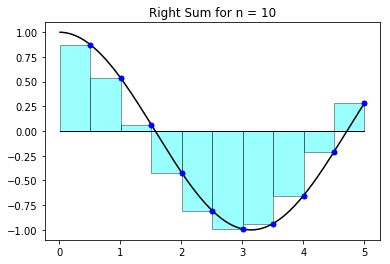
\includegraphics[width=0.9\linewidth]{RiemannSumN10.png}
  \caption{n=10}
\end{subfigure}
\begin{subfigure}{.33\textwidth}
  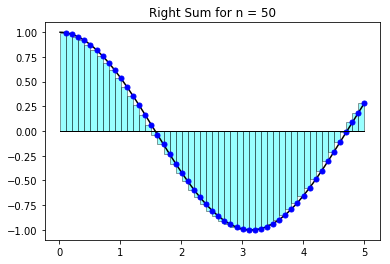
\includegraphics[width=0.9\linewidth]{RiemannSumN50.png}
  \caption{n=50}
\end{subfigure}
\caption{Upper Riemann Sums for $\cos(x)$ on $[0,5]$ using $n$ subintervals of equal length.}
\label{fig:RiemannSumIncresN}
\end{figure}


Notice each term in this sum is of the form $f(x)(x_i-x_{i-1})$, this is the area of a rectangle with height $f(x)$ and width $(x_i-x_{i-1})$. In the case of the upper sum, we take the value of $f$ at rightmost end point of the interval $[x_{i-1},x_i]$ with the left most value of the interval being used for the lower sum. If we want a function to have a definite area under it, we'd expect that the upper and lower sums fo become closer and closer as the mesh of our partition decreases since the left endpoint will approach the right endpoint of each interval. Since we'd want the intervals to be `infinitely' thin to ensure accuracy, this motivates us to define the integral in terms of limits.

\subsection{Definite Integrals}

\begin{defn}[Definition of the Definite Integral]\label{DefInt}
We define the \emph{(definite) integral of $f$ over $[a,b]$} to be
\begin{equation}
  \int_{a}^{b}f(x)dx\coloneqq \lim\limits_{\norm{P}\to 0}U(f;P)=\lim\limits_{\norm{P}\to 0}L(f;P)
\end{equation}
provided both limits exist and are equal. That is, the integral is the defined as the limit of our Riemann sum as the number of rectangles goes to infinity and each becomes infinitely thin having infinitesimal width $dx$.
\end{defn}
\begin{rem}
When the integral as defined above exists, we say that $f$ is \emph{integrable} on $[a,b]$.
\end{rem}

This raises the question of what kinds of functions are integrable for this. To provide a partial answer, we have the following proposition.
\begin{prop}\label{IntExists}
    When the function $f$ is continuous on $[a,b]$, the integral $\int_{a}^{b}f(x)dx$ exists.
\end{prop}
Though we know that every continuous function is integrable, we also know that not every function is integrable.

%% Might want to recycle this for blog post.
Notice that the limit in \cref{DefInt} is independent of partition so that if we have a sequence of partitions $P_n$ whose mesh go to 0, then we can compute the integral of $f$, so that
\begin{equation}\label{RegPartLim}
  \int_{a}^{b}f(x)dx=\lim\limits_{n\to\infty}U(f;P_n)=\lim\limits_{n\to\infty}L(f;P_n).
\end{equation}
\begin{exmp}
Suppose we want to calculate the integral of $f(x)=x^2$ on $[0,1]$. By cref{IntExists}, we can know $\int_{0}^{1}x^2dx$ exists and  pick sequence of partitions $P_n$ where each partition is given by
\begin{equation}
  P_n=\left\{0, \frac{1}{n}, \frac{2}{n},\dotsc, \frac{n-1}{n}, 1 \right\}=\left\{\frac{i}{n}\mid 0\leq i\leq n\right\},
\end{equation}
dividing $[0,1]$ into $n$ subintervals of equal length.
Since $\norm{P}$ is clearly $\frac{1}{n}$, we can write the upper Riemann sum as
\begin{equation}
  U(f;P_n)=\sum_{i=1}^{n}f\left(\frac{i}{n}\right)\left(\frac{i}{n}-\frac{i-1}{n}\right)=\sum_{i=1}^{n}\frac{i^2}{n^2}\left(\frac{1}{n}\right)=\frac{1}{n^3}\sum_{i=1}^{n}i^2.
\end{equation}
Using \cref{IntegerSums} we can reduce the above equations to
\begin{equation}
  U(f;P_n)=\frac{n(n+1)(2n+1)}{6n^3}=\frac{1}{3}+\frac{3}{n}+\frac{1}{n^2}.
\end{equation}
Taking the limit, we see that $\int_{0}^{1}x^2dx=\frac{1}{3}$ by (\ref{RegPartLim}).
\end{exmp}

This process can be visualized using computer code as in \cref{fig:RiemannSumIncresN}. Though we can use Riemann sums to solve for the integrals of simple functions directly, this method is tedious and doesn't always come easily. Therefore, we will need to develop some method of easily computing integrals, but first we must establish some more properties of the integral.

\begin{lem}[Linearity of the Integral]
The integral is linear in the following sense: For any integrable $f$ and $g$ on $[a,b]$,
\begin{enumerate}
  \item $\int_{a}^{c}f(x)dx+\int_{c}^{b}f(x)dx$ if $a<c<b$,
  \item $\int_{a}^{b}[f(x)+g(x)]dx=\int_{a}^{b}f(x)dx+\int_{a}^{b}g(x)dx$,
  \item $\int_{a}^{b}c f(x)dx=c\int_{a}^{b}f(x)dx$ for any constant $c$.
  \item $\int_{a}^af(x)dx=0$
  \item $\int_{a}^{b}f(x)dx=-\int_{b}^{a}f(x)dx$.
\end{enumerate}
\end{lem}
\begin{rem}
  Notice that the first three properties mirror those of the sum that we presented in \cref{LinSum}.
\end{rem}
A consequence of this similarity is that the sum \emph{commutes} with the integral.
\begin{cor}\label{SumIntCom}
  If $f_1, f_2, \dotsc, f_n$ are integrable functions on $[a,b]$, then
  \begin{equation}
    \int_{a}^{b}\left(\sum_{i=1}^{n}f_i(x) \right)dx= \sum_{i=1}^{n}\left(\int_{a}^{b}f_{i}(x)dx\right).
  \end{equation}
\end{cor}
We can restate \cref{SumIntCom} as ``the sum of the integral is the integral of the sum''. Furthermore, we can deduce more properties of the integral  such the integral of a non-negative function must be non-negative. With this in mind, we can get a very crude bound on the definite integral of a function.

%%%% Add other properties as exercises

\begin{prop}
  If $f$ is an integrable function on $[a,b]$ and $m$ and $M$ the minimum and maximum on $[a,b]$ respectively, then
  \begin{equation}
    m(b-a)\leq \int_{a}^{b} f(x)dx\leq M(b-a).
  \end{equation}
\end{prop}
\begin{rem}\label{ConstInt}
  This immediately tells us that for any constant function $c$ on $[a,b]$, $\int_{a}^{b} c\ dx=c(b-a)$.
\end{rem}

\section{Fundamental Theorems of Calculus}

%% Include applications of FTC, physics? Basic Mechanics. position, velocity, acceleration, starting from velocity function.

%% Add useful examples for each of the techniques!!


%% u-sub Expectation of Exponential distribution? Frame in terms of chemical decay / half life? Expectation of normal distribution

%% LIATE for IBP

%% Derivation of Taylor's formula by IBP (https://math.stackexchange.com/questions/20397/striking-applications-of-integration-by-parts) maybe save for Taylor's theorem or as a hint for it

%% IBP: Gamma function and acting like factorial, provide history on it


%% Later chapter: intro to Fourier Series pair with Taylor's theorem


\subsection{Indefinite Integrals}


In general, we want to be able to compute the actual value of the integral in an easy way, not just establish a crude estimate or use Riemann sums to compute the value as it can be tedious or impossible. In order to make the process of finding integrals easier, we'll begin to establish a relationship between differentiation and integration. We'll start with the notion of an anti-derivative.
\begin{defn}[Anti-derivative]
If $f$ is a function on $[a,b]$, we say that a differentiable function $F$ is an \emph{anti-derivative} if $F'(x)=f(x)$ for all $x\in [a,b]$.
\end{defn}
\begin{prop}\label{PlusC}
  If $F$ is an anti-derivative of $f$, then $F(x)+C$ is also an anti-derivative of $f$ for any constant $C$. Moreover, if $F_1$ and $F_2$ are anti-derivatives, then they differ by a constant.
\end{prop}
\begin{proof}
  Since the derivative of any constant $C$ is $0$, the derivative of $F$ must equal the derivative of $F(x)+C$. Similarly, if $F_1$ and $F_2$ are two anti-derivatives of $f$, then $F_1-F_2$ must have derivative 0. Therefore, their difference is constant, so that $F_1(x)=F_2(x)+C$ for some $C$.
\end{proof}

\begin{defn}[Indefinite Integral]
With \cref{PlusC} in mind, we define the \emph{indefinite integral of $f$} as
\begin{equation}
  \int f(x)dx\coloneqq F(x)+C,
\end{equation} where $F$ is an anti-derivative of $f$. We use $C$ as placeholder constant to denote all positive anti-derivatives of f.
\end{defn}

Armed with this, we can now state one of the two Fundamental theorems of calculus.

\begin{thm}[The First Fundamental Theorem of Calculus]\label{FundThmOne}
  Suppose $f$ is a continuous function on the interval $[a,b]$. If we define \begin{equation}
    F(x)=\int_{a}^x f(t)dt,\text{ then } F'(x)=f(x),
  \end{equation}
  i.e. $\int_{a}^x f(t)dt$ is an anti-derivative of $f(x)$.
\end{thm}
Therefore, any continuous function of an interval has an anti-derivative on that interval.
\begin{thm}[The Second Fundamental Theorem of Calculus]\label{FundThmTwo} If $f$ is integrable on $[a,b]$, then \begin{equation}\label{FTC2}
  \int_{a}^{b}f(x)dx=F(b)-F(a)
\end{equation}for any anti-derivative $F$.
\end{thm}
\begin{rem}
  Notice that the Second Fundamental Theorem of Calculus is independent of our choice of anti-derivative by \cref{PlusC}, so we can always set $C=0$. That is, provided $F$ exists. We will often use $\eval{F(x)}_{a}^{b}$ as shorthand for $F(b)-F(a)$, emphasizing the relationship between the indefinite and definite integrals.
\end{rem}

\cref{FundThmOne} and \cref{FundThmTwo} are called the Fundamental Theorems of Calculus (FTC for short) because they establish the relationship between differentiation and integration. The idea being that the derivative and integration are functionally opposite operatives. One immediate result of the \cref{FundThmTwo} is that we have drastically simplified the problem of computing the definite integral; we simply need to find an anti-derivative.\\

The Fundamental Theorems of Calculus make the problem of finding the definite integral of functions like $f(x)=x$ much simpler as we can compute that
\begin{equation}
  \int_{a}^{b}x\ dx=\frac{b^2}{2}-\frac{a^2}{2}
\end{equation}
since $\frac{x^2}{2}$ is an anti-derivative of $x$. In fact, we can easily derive a more general statement for the indefinite integral of powers of $x$.

\begin{prop}[Reverse Power Rule]\label{RevPowRule}
  If $f(x)=x^n$ for some $n\neq -1$, then $f$ has anti-derivative $F(x)=\frac{x^{n+1}}{n+1}$ i.e
  \begin{equation}
    \int x^n\ dx=\frac{x^{n+1}}{n+1}+C.
  \end{equation}
\end{prop}

\begin{rem}
  In particular, this shows that for any constant $c=cx^0$, we have $\int c\ dx=cx$ which is consistent with \cref{ConstInt}.
\end{rem}

Using the linearity of the integral, we can use \cref{RevPowRule} to derive a formula for the indefinite integral (or anti-derivative) of any polynomial.
\begin{cor}\label{PolyInt}
If we have a polynomial $p(x)=a_nx^n+a_{n-1}x^{n-1}\dotsb+a_1x+a_0$ where the $a_i$ are constants, then
\begin{equation}
  \int p(x)dx= \left(\frac{a_n}{n+1}\right)x^{n+1}+ \left(\frac{a_{n-1}}{n}\right)x^{n}+\dotsb+\left(\frac{a_1}{2}\right)x^2+a_0x+C.
\end{equation}
\begin{proof}
  Writing our polynomial as $p(x)=\sum_{i=0}^{n}a_ix^i$ using sum notation, we can use \cref{SumIntCom} to see that
  \begin{equation}
    \int p(x)dx= \int \left(\sum_{i=0}^{n}a_ix^i\right)dx=\sum_{i=0}^{n}\left( \int a_ix^i dx \right).
  \end{equation}
  Therefore, we can use \cref{RevPowRule} to compute the integral on the righthand side, so that
  \begin{equation}
      \int p(x)dx=\sum_{i=0}^{n}\left( \frac{ a_i}{i+1}\right) x^{i+1}+C.
  \end{equation}
\end{proof}
\end{cor}

\subsection{Consequences of the Fundamental Theorems}

%% Need more expositon. Examples after each theorem.

We can derive similar formulas for the integrals of the trigonometric functions with
\begin{equation}
  \int\sin(x)\ dx= -\cos(x)+C
 \text{ and }   \int_{a}^{b}\cos(x)\ dx=\sin(x)+C,
\end{equation}
which for now we will take as granted.

%% This follows from the theorem I proved earlier... \href{SinCosExpDif} so it's not for granted. Pls fix.

%% We have this example, but what if we're dealing with a function like \sin x \cos x

%% has anti-derivatives \sin^2 and  -\cos^2x

We can also define formulas for the integrals composition of functions.

\begin{thm}[$u$-Substitution]\label{USub}
  For functions $f,u$ such that $u$ is differentiable on $[a,b]$ and $f$ is continuous on the image $u([a,b])$,
  \begin{equation}
    \int_{a}^{b}f(u(x))u'(x)dx=\int_{u(a)}^{u(b)}f(x)dx.
  \end{equation}
\end{thm}

\begin{proof}
  Since $f$ is continuous, it has an anti derivative $F$. Noticing that $F\circ u$ has derivative $F'(u(x))u'(x)$ by chain rule, we see that $F\circ u$ is an anti derivative of $f(u(x))u'(x)$. Therefore, \cref{FundThmTwo} tells us that
  \begin{equation}
      \int_{a}^{b}f(u(x))u'(x)dx=F(u(b))-F(u(a))=\int_{u(a)}^{u(b)}f(x)dx.
  \end{equation}
\end{proof}
\begin{rem}
  There is an direct analogue of this for indefinite integrals which we will use later.
\end{rem}

Notice this resembles the chain rule, but in reverse. This allows us to reduce integrals of many functions into the cases we've described above. Similarly, we can prove a sort of reverse product rule.

%% Completing the example above


%% What if we can write the problem in terms of a derivative and a function... product of two (incapatible) functions. For example, $x^2 e^x$

\begin{thm}[Integration by Parts]\label{IBP}
For differentiable functions $u,v$ on $[a,b]$,
\begin{equation}
  \int_{a}^{b}u\ dv=\eval{(uv)}^{b}_{a}-\int_{a}^{b}v\ du.
\end{equation}
where $dv$ and $du$ denote $v'(x)dx$ and $u'(x)dx$ respectively.
\end{thm}
\begin{proof}
  Consider the function $u\cdot v$. By the product rule, its derivative is $uv'+vu'$. Therefore, linearity of the integral and FTC tell us
  \begin{equation}
  \eval{(uv)}^{b}_{a}= \int_{a}^{b}[u(x)v'(x)+v(x)u'(x)]dx=\int_{a}^{b}u(x)v'(x)dx + \int_{a}^{b}v(x)u'(x)dx.
\end{equation}
Making the substitutions $dv=v'(x)dx$, $du=u'(x)dx$ and subtracting over the second term, we get the result
\begin{equation*}
  \int_{a}^{b}u\ dv=\eval{(uv)}^{b}_{a}-\int_{a}^{b}v\ du.
\end{equation*}
\end{proof}

%% Write function to draw integrals for the symmetric case.
Furthermore, we can see that integral is consistent with our geometric intuition of area under the curve when it comes to functions with symmetry.
\begin{prop}[Integrating Even and Odd Functions]\label{SymInt}
  Suppose $f$ is continuous on $[-b, b]$, then
  \begin{align}
    \int_{-b}^{b}f(x)dx&=2\int_{0}^{b}f(x)dx \text{ if  $f$ is even, and}\\
    \int_{-b}^{b}f(x)dx&=0  \text{ if  $f$ is odd}.
  \end{align}
\end{prop}

\begin{prop}[Integrating Periodic Functions]\label{PerInt}
  If $f$ is continuous and periodic with period $T$, then \begin{equation}
      \int_{x}^{x+T}f(x)dx=\int_{0}^{T}f(x)dx \text{ for any $x$.}
  \end{equation}
\end{prop}

We can use these to compute the followings examples. %% Do several practice integrals.
\begin{exmps}

Compute the indefinite integral $\int f(x)dx$ for the following functions:
\begin{enumerate}[label=\textbf{Example A.\arabic*.}]
  \addtolength{\itemindent}{1.625cm} % move right
  \item \label{IntEA1} $f(x)=x^5+2x+1$, %% Hint: \cref{PolyInt}
  \item \label{IntEA2} $f(x)=\cos(x)\sin^2(x)$, %% Hint:\cref{USub}
  \item \label{IntEA3} $f(x)= \sin^2(x)+\cos^2(x)$, %% Trig
  \item \label{IntEA4} $f(x)=\frac{3x}{\sqrt{x^2+1}}$, %%\cref{USub}+\\ref{RevPowRule}
  \item \label{IntEA5} $f(x)= 3x\cos(x)$ %%\cref{IBP}
\end{enumerate}

Starting with \ref{IntEA1}, we can see that this is an application of \cref{PolyInt}, so that
\[
\int (x^5+2x+1)\ dx=\frac{x^6}{6}+x^2+x+C.
\]

For \ref{IntEA2}, we'll need $u$-substitution. Noticing that the derivative of $\sin^2(x)$ will have a $\cos(x)$ in front by Chain Rule ($\diff{}{x}(\sin x)=\cos x$), we define $u=\sin(x)$ so that $du=\cos(x)dx$. Therefore, we can make these substitutions and see
\[
\int \cos(x)\sin^2(x)dx=\int \underbrace{\sin^2(x)}_{u^2}\underbrace{\cos(x)dx}_{du}=\int u^2du= \frac{1}{3}u^3+C.
\]
To finish, we have to back substitute, so that everything is in terms of $x$, so our final answer is
\[
\int \cos(x)\sin^2(x)dx=\frac{1}{3}\sin^3(x)+C.
\]
\ref{IntEA3} comes down to the trig identity $\sin^2(x)+\cos^2(x)=1$, so that
\[
\int \sin^2(x)+\cos^2(x) dx= \int 1\ dx= x+C.
\]

Moving onto \ref{IntEA4}, we see that the function $x^2+1$ has derivative $2x$, so we can try $u$-substitution again. Making the substitution $u=x^2+1$, we get $du=2x$, so that $\frac{3}{2}du=3x\ dx$. Therefore, making these substitutions, we compute
\begin{align}
  \int \frac{3x}{\sqrt{x^2+1}}\ dx=\frac{3}{2}\int\frac{1}{\sqrt{u}}du& =\frac{3}{2}\int u^{-\frac{1}{2}}du\\
  &= \frac{3}{2}\cdot2u^{\frac{1}{2}}+C, \text{ by \cref{RevPowRule}}\\
  &= 3(x^2+1)^{\frac{1}{2}}+C, \text{ back substituting }u=x^2+1.
\end{align}

We can see that \ref{IntEA5} is the product of two functions, neither of which contains the derivative of the other, so $u$-substitution will not work. Therefore, we try the product rule. Letting, $u=3x$ and $dv'=\cos(x)$, we have $u'=3$ and $v=\sin(x)$. Plugging this into the formula, we get
\[
\int 3x\cos(x)dx= 3x\sin(x)-\int 3\sin(x)dx=3x\sin(x)-3\cos(x)+C.
\]
\\

Let's try to do the same for definite integrals.

Compute the definite integral $\int_{a}^{b} f(x)$ for the following functions:
\begin{enumerate}[label=\textbf{Example B.\arabic*.}]
  \addtolength{\itemindent}{1.625cm} % move right
  \item \label{IntEB1} $f(x)=x^3, a=-2, b=4$
  \item \label{IntEB2} $f(x)=\sin^{5001}(x), a=-1, b=1$, %% Hint: Odd
  \item \label{IntEB3} $f(x)=4x(x^2+8)^3$,               %% Hint: u-sub
  \item \label{IntEB4} $f(x)=\sin(x)\cos^2(x), a=-\frac{3\pi}{2},b=\frac{5\pi}{2}$ %% Hint: u-sub/odd
  \item \label{IntEB5} $f(x)=\abs{\cos(x)}, a=0, b=2000\pi$ %% Hint: Even
\end{enumerate}

Starting with \ref{IntEB1}, we can see this is just an application of the reverse power rule, so that
\[
\int_{-2}^{4}x^3=\eval{\left(\frac{x^4}{4}\right)}^{4}_{-2}=\frac{4^4}{4}-\frac{(-2)^4}{4}=64-4=60.
\]

\ref{IntEB2} looks to be ridiculously hard to solve directly. We'll need to be clever here. Noticing that $\sin x$ is odd and that, therefore, $\sin^{5001}(x)$ must be odd, we can use this symmetry as in \cref{SymInt} to see that $\int_{-1}^{1} \sin^{5001}(x)dx=0$.\\


\ref{IntEB3} and \ref{IntEB4} are applications of $u$-substitution and will be left as exercises.

Lastly, \ref{IntEB5} can be solved using the periodic of $\abs{\cos (x)}$. Since $\abs{\cos (x)}$ has period $\pi$, we can decompose the integral as
\[
\int_{0}^{2000\pi}\abs{\cos(x)}dx=2000\int_{0}^{\pi}\abs{\cos(x)}dx
\]
using \cref{PerInt}. This leaves us to calculate $\abs{\cos(x)}$. Since $\cos(x)$ is non-negative on $[0,\frac{\pi}{2}]$ and negative on $[\frac{\pi}{2}, \pi]$, we can once again decompose the integral to find
\[
\int_{0}^{\pi}\abs{\cos(x)}dx= \int_{0}^{\frac{\pi}{2}}\cos(x)dx-\int_{\frac{\pi}{2}}^{\pi}\cos(x)dx=\eval{\sin(x)}_{0}^{\frac{\pi}{2}}-\eval{\sin(x)}_{\frac{\pi}{2}}^{\pi}=2\sin\left(\frac{\pi}{2}\right)=2.
\]
Therefore, our final answer is
\[
\int_{0}^{2000\pi}\abs{\cos(x)}dx=4000.
\]
\end{exmps}


With our knowledge that differentiation and integration are a kind of reciprocal operations via the FTC, we can prove an analogue of the Mean Value theorem for integrals.
\begin{thm}[Mean Value Theorem for Integrals]
  If $f$ is continuous on $[a,b]$, then there exists some point $c$ in $[a,b]$ such that
  \begin{equation}
    f(c)=\frac{1}{b-a}\int_{a}^{b}f(x)dx.
  \end{equation}
\end{thm}
\begin{proof}
  Since $f$ is continuous, we have an anti-derivative $F(x)=\int_{a}^{x}f(t)dt$ which is differentiable on $(a,b)$ and continuous on $[a,b]$. Therefore, the Mean Value theorem for derivatives (\cref{MVTD}) states there is some $c$ such that
  \begin{equation}
    F'(c)=\frac{1}{b-a}\big(F(b)-F(a) \big).
  \end{equation}
  Since $F$ is an anti-derivative of $f$ and $\int_{a}^{a}f(t)dt=0$, we have
\begin{equation}
  f(c)=F'(c)=\frac{1}{b-a}\left( \int_{a}^{b}f(t)dt-\int_{a}^{a}f(t)dt \right)=\frac{1}{b-a}\int_{a}^{b}f(x)dx.
\end{equation}
\end{proof}
\begin{rem}
  The Mean Value Theorem for integrals gives a way of finding the average value of a function over an interval. The integral of $f$ amounts to summing up all the values $f$ on the interval $[a,b]$, then the factor of $\frac{1}{b-a}$ accounts for length of the interval that we summed over.
\end{rem}

Now that we've a solid grounding in how integration works and some of its important tools, we'll move to the kinds of problems in which integration can be applied.
\section{Applications of Integration}

%%% Solids of revolution, write code for visualizing this.

\subsection{Area \& Solids of Revolution}

\subsection{Mechanics}

\subsection{Arc Length}


%% Improper Integrals

\section{Special Functions}

\subsection{Exponentials and Logarithms}

\subsection{Improper Integrals}
%%% Relation to distribution functions.

%%% Euler's and computation

%%% L'Hopital's

\section{Sequences and Series}
% Sequences, Sums and Series,

\subsection{Convergence Tests}

\subsection{Power Series and Taylor's Theorem}
%% Power Series, Taylor's Theorem

%%Appendix on computation / numerical methocs

\end{document}
